\section{Single Phase Half Wave Uncontrolled Rectifier with RL load and Freewheeling Diode}

\subsection{Circuit used for simulation}

% figure that is centered on the page
\begin{figure}[h]
    \centering
    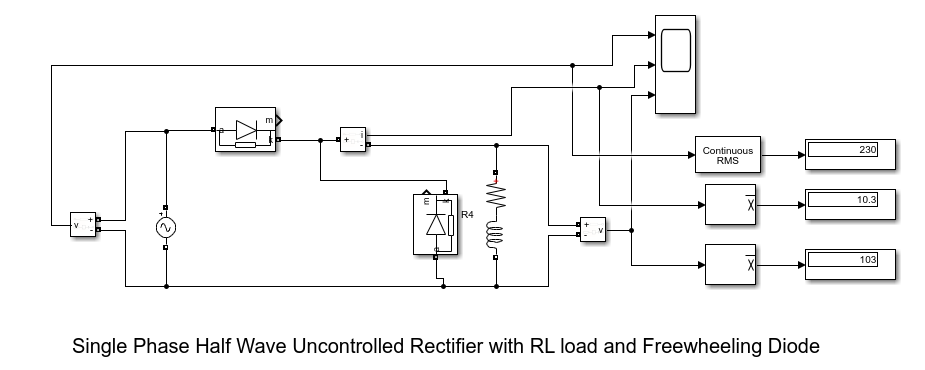
\includegraphics[width=0.7\textwidth]{images/experiment-1/circuit-diagram-simulation-03.png}
    \caption{Circuit used for simulation}
    \label{Fig_simulation_circuit_single-phase-half-wave-uncontrolled-rectifier-with-RL-load-and-freewheeling-diode}
\end{figure}

\subsection{Components Required}

\begin{table}[h]
    \renewcommand{\arraystretch}{1.3}
    \label{table_components_required_circuit_3}
    \centering
    \begin{tabular}{|c|c|c|c|}
        \hline
        Sr. No & Parameters                     & Ratings            & Quantity \\
        \hline
        \hline
        1      & AC Single Phase Voltage Source & 230V ($ V_{rms} $) & 1        \\
        \hline
        2      & Resistor                       & 10$ \Omega $       & 1        \\
        \hline
        3      & Inductor                       & 10mH               & 1        \\
        \hline
        4      & Diode                          & -                  & 1        \\
        \hline
        5      & Voltmeter                      & -                  & 2        \\
        \hline
        6      & Ammeter                        & -                  & 1        \\
        \hline
    \end{tabular}
    \caption{Components for Single Phase Half Wave Uncontrolled Rectifier with RL load and Freewheeling Diode}
\end{table}


\subsection{Observations}

\begin{table}[h]
    \renewcommand{\arraystretch}{1.3}
    \label{table_observation_3}
    \centering
    \begin{tabular}{|c|c|c|}
        \hline
        Parameters                              & Theoretical Values & Simulation Values \\
        \hline
        \hline
        AC Input Voltage ($ V_{in,rms} $)       & 230V               & 230V              \\
        \hline
        Output Average Voltage ($ V_{o,avg} $)  & 103.53V            & 103V              \\
        \hline
        Output Average Current ($ I_{o,avg}  $) & 10.35A             & 10.3A             \\
        \hline
        AC Input Power ($ P_{AC}  $)            & 2389.5 (W)         & 2404 (W)          \\
        \hline
        DC Input Power ($ P_{DC}  $)            & 1071.53 (W)        & 1061 (W)          \\
        \hline
        Efficiency (\%)                         & 44.84              & 44.13              \\
        \hline
    \end{tabular}
    \caption{Observations for Single Phase Half Wave Uncontrolled Rectifier with RL load and Freewheeling Diode}

\end{table}



Upon analysis, it has been observed that the simulated output voltage closely approximates the calculated voltage, whereas the simulated output current significantly deviates from the calculated current. The incorporation of the freewheeling diode results in a sudden cessation of output current in the rectifier circuit when the AC supply source drops to zero volts, as the lagging current shifts to flow through the freewheeling diode rather than the rectifier circuit.
The efficiency of uncontrolled rectifier with RL load with freewheeling diode is 44.13\%.

\pagebreak

\subsection{Resultant Waveforms}


% figure that is centered on the page
\begin{figure}[h]
    \centering
    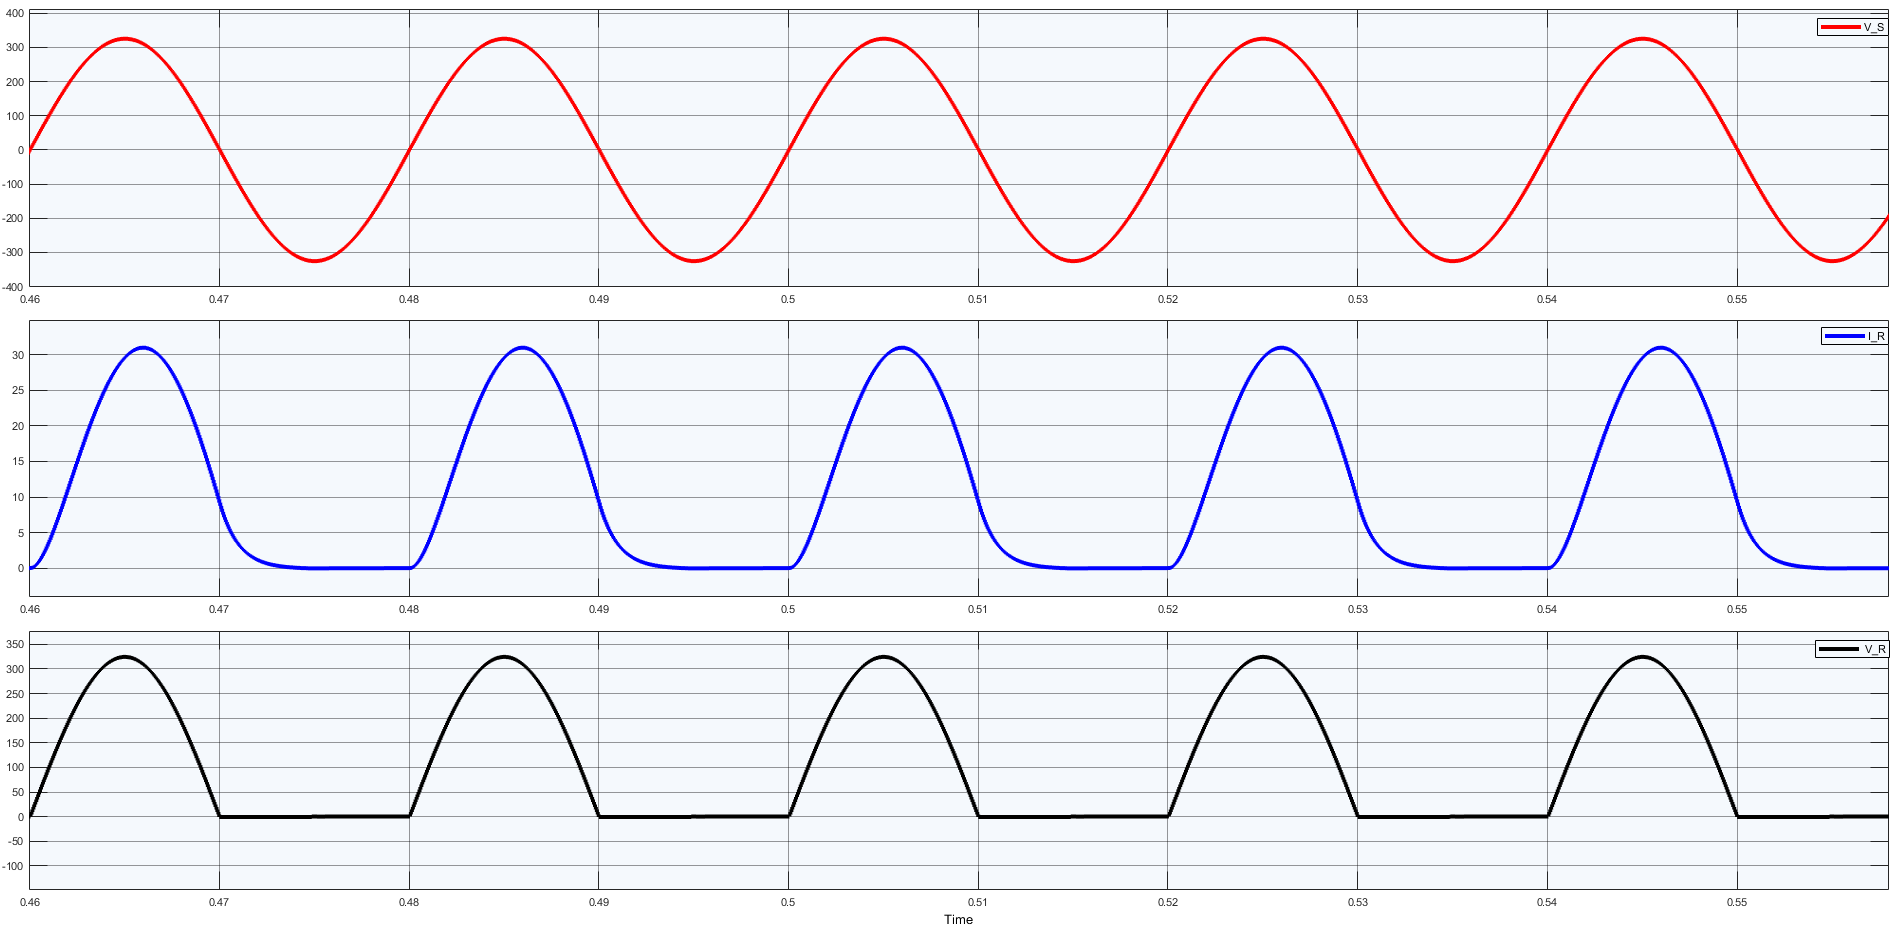
\includegraphics[width=1\textwidth]{images/experiment-1/circuit-scope-simulation-03.png}
    \caption{Scope Waveforms for Single Phase Half Wave Uncontrolled Rectifier with RL load and Freewheeling Diode}
    \label{Fig_waveform_single-phase-half-wave-uncontrolled-rectifier-with-RL-load-and-freewheeling-diode}
\end{figure}


\pagebreak

